% !TEX TS-program = pdflatex
% !TEX encoding = UTF-8 Unicode

% This is a simple template for a LaTeX document using the "article" class.
% See "book", "report", "letter" for other types of document.

\documentclass[11pt]{report} % use larger type; default would be 10pt

\usepackage[utf8]{inputenc} % set input encoding (not needed with XeLaTeX)
\usepackage{multirow}

%%% Examples of Article customizations
% These packages are optional, depending whether you want the features they provide.
% See the LaTeX Companion or other references for full information.

%%% PAGE DIMENSIONS
\usepackage{geometry} % to change the page dimensions
\geometry{a4paper} % or letterpaper (US) or a5paper or....
% \geometry{margin=2in} % for example, change the margins to 2 inches all round
% \geometry{landscape} % set up the page for landscape
%   read geometry.pdf for detailed page layout information

\usepackage{graphicx} % support the \includegraphics command and options

% \usepackage[parfill]{parskip} % Activate to begin paragraphs with an empty line rather than an indent

%%% PACKAGES
\usepackage{booktabs} % for much better looking tables
\usepackage{array} % for better arrays (eg matrices) in maths
\usepackage{paralist} % very flexible & customisable lists (eg. enumerate/itemize, etc.)
\usepackage{verbatim} % adds environment for commenting out blocks of text & for better verbatim
\usepackage{subfig} % make it possible to include more than one captioned figure/table in a single float
% These packages are all incorporated in the memoir class to one degree or another...

%%% HEADERS & FOOTERS
\usepackage{fancyhdr} % This should be set AFTER setting up the page geometry
\pagestyle{fancy} % options: empty , plain , fancy
\renewcommand{\headrulewidth}{0pt} % customise the layout...
\lhead{}\chead{}\rhead{}
\lfoot{}\cfoot{\thepage}\rfoot{}

%%% SECTION TITLE APPEARANCE
\usepackage{sectsty}
\allsectionsfont{\sffamily\mdseries\upshape} % (See the fntguide.pdf for font help)
% (This matches ConTeXt defaults)

%%% ToC (table of contents) APPEARANCE
\usepackage[nottoc,notlof,notlot]{tocbibind} % Put the bibliography in the ToC
\usepackage[titles,subfigure]{tocloft} % Alter the style of the Table of Contents
\renewcommand{\cftsecfont}{\rmfamily\mdseries\upshape}
\renewcommand{\cftsecpagefont}{\rmfamily\mdseries\upshape} % No bold!

%%% END Article customizations

%%% The "real" document content comes below...

\title{NaoCar}
\author{Samuel Olivier\and
Gaël du Plessix\and
Melvin Laplanche\and
Loick Michard}

%\date{} % Activate to display a given date or no date (if empty),
         % otherwise the current date is printed 

\begin{document}
\maketitle
\tableofcontents

\chapter{Contexte}
	\section{Bilan de la technologie}
		Depuis quelques années, la recherche en matière de robotique a tendance à évoluer en direction des robots humanoïdes.
		En effet, les chercheurs visent à construire des robots effectuant toutes les actions qu'un humain est capable de réaliser.
		Notamment marcher sur deux jambes, attraper des objets, parler, communiquer ou même conduire...\\
		La recherche en robotique a pour objectif final d'assister l'humain dans les taches quotidiennes, voire de le remplacer.\\\\
		\begin{figure}[htb]
			\centering
			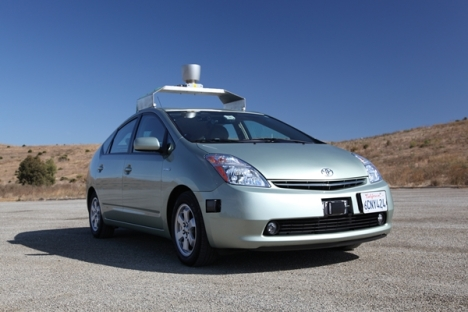
\includegraphics[scale=1]{google-car.jpeg}
			\caption{Google self driving car}
			\label{fig:google-car}
		\end{figure}
	\newpage
	\section{Un projet étudiant}
		\subsection{Description du projet}
			\begin{figure}[htb]
			\centering
			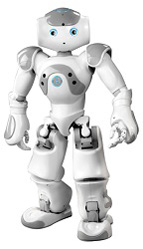
\includegraphics[scale=0.2]{nao2.jpg}
			\caption{NAO}
			\label{fig:nao}
			\end{figure}
		Le projet NaoCar s'inspire de projets de conduite autonome, comme la google self-driving car. La différence majeure par rapport aux projets existant est le fait que la voiture soit pilotée par un robot humanoide: Nao. Celui-ci place l'intéraction homme-machine au centre du projet. Grâce à ces nombreux capteurs et servomoteurs, il devra être capable de piloter une voiture miniature adaptée avec une autonomie maximale.
		\subsection{PFA}
			Notre projet s'inscrit dans le cadre de la 3ème année à Epitech. Il se déroule pendant un an, incluant plannification, organisation, recherche de partenaires et développement du projet.\\
			
	\section{Une vision d'avenir}
			Le projet NaoCar se positionne dans la continuité des recherches actuelles, qui visent à amincir les frontières entre l'homme et la machine. En l'occurence, permettre à Nao de conduire une voiture pour enfant démontrerait de sa capacité à intéragir de manière transparente avec des objets conçus pour l'homme.
\chapter{Définition des objectifs}
	\section{Les objectifs techniques}
		\subsection{Contrôle et déplacement du robot}
			Le robot Nao doit être capable de manipuler les commandes de sa voiture afin d'effectuer les actions suivantes:
\begin{itemize}
\item Avancer
\item Reculer
\item Tourner à gauche
\item Tourner à droite
\end{itemize}
			Dans ce but, compte tenu de la configuration de son véhicule, Nao doit pouvoir:
\begin{itemize}
\item Actionner le levier de vitesse en position "avancer"
\item Actionner le levier de vitesse en position "reculer"
\item Tourner le guidon à gauche
\item Tourner le guidon à droite
\item Appuyer sur la pédale d'accélération
\end{itemize}
			Le robot doit pouvoir être contrôlé de manière très simple, via une interface proposant simplement les quatres actions avancer, reculer, tourner à gauche et tourner à droite.\\
			Ce contrôle devra pouvoir être effectué depuis un ordinateur et/ou un appareil mobile (smartphone/tablette) connecté sur le même réseau que le robot. On pourra aussi visualisé ce que voit Nao via cette même interface.
		\newpage
		\subsection{Intelligence artificielle: conduite autonome}
			\subsubsection{Conduite et reconnaissance de formes}
				Dans un premier temps, nao doit etre capable de pouvoir conduire en suivant une ligne de couleur ou une piste différenciable
			\subsubsection{Vers une conduite en totale autonomie}
				Dans un second temps, Nao doit pouvoir:
				\begin{itemize}
				\item Integrer la Kinect dans NaoCar
				\item Detecter les obstacles
				\item Éviter les obstacles
				\end{itemize}
		\subsection{Matériel}
			Le véhicule utilisé sera une voiture pour enfant légèrement modifiée afin de pouvoir être pilotée par Nao. La voiture retenue se déplace à une vitesse de 3 km/h et dispose d'un faible angle de braquage. Cette première solution permettra de concevoir les solutions logicielles de pilotage et de conduite autonome afin de réaliser un premier prototype.\\
	\section{Communication autour du projet}
		\subsection{Évènements}
			\subsubsection{Foire exposition de Montpellier}
				\begin{figure}[htb]
				\centering
				
\includegraphics[width=1\textwidth]{foire-expo.png}
				\caption{Foire Expo Montpellier}
				\label{fig:Foire Expo Montpellier}
				\end{figure}
				La foire expositons internationale de Montpellier est un évènement de choix pour présenter le projet NaoCar au public pour la première fois.
				Installée au Parc des Expositions de Montpellier, cet évènement constitu la première démonstration publique du projet. Il permettra de tester la réaction à un public non-initié face aux différentes démontrations.
			\subsubsection{Montpellier In Game}
				\begin{figure}[htb]
				\centering
				
\includegraphics[width=1\textwidth]{mig.png}
				\caption{Montpellier In Game}
				\label{fig:Montpellier In Game}
				\end{figure}
	                        Le MIG est "un rendez-vous original pour l’industrie du jeu vidéo proposant à la fois des rencontres professionnelles de haut niveau et un grand salon populaire". \\Cet évènement se place donc dans les dates clés de notre projet en matière de promotion et de communication afin de pouvoir avoir des contacts avec les professionnels intéressés. Ce salon permettra aussi de tester la réaction d'un public initié aux nouvelles technologies.
			L'objectif principal est d'obtenir un maximum de visite sur le stand du projet NaoCar.
		\newpage
	                \subsubsection{Salon de l'étudiant de Montpellier}
				\begin{figure}[htb]
				\centering
				
\includegraphics[width=0.5\textwidth]{salon-de-l-enseignement-superieur-de-montpellier.jpg}
				\caption{Salon de l'etudiant de Montpellier}
				\label{fig:Salon de l'etudiant de Montpellier}
				\end{figure}
				Ce salon réunit un grand nombre de personnes voulant en apprendre plus sur les différents établissements scolaires. Par conséquent, en plus de promouvoir le projet, nous aurons également l'occasion de se créer des contacts avec des écoles qui pourraient prendre part au projet dans certains domaines que nous ne pouvons pas couvrir.
		\subsection{Partenariat}
			Afin de travailler dans de meilleures conditions nous envisageons divers partenariats, et plus particulièrement un partenariat avec un concessionaire automobile qui serai apte à nous fournir une voiture de meilleure qualité.
		\subsection{Vidéos de promotion}
			Des vidéos de promotion devront être réalisées et diffusées sur les réseaux sociaux ainsi que sur différentes plateformes de streaming, afin faire connaitre le projet au plus de personnes possible, et ainsi d'améliorer les chances de partenariats.\\
			Notre objectif est de réaliser plus de 3 000 vues.
		\subsection{Ouverture à la communauté}
			Les sources du projet sont disponibles sur Github sous licence libre, ce qui permet à toutes les personnes intéressées d'utiliser et de modifier NaoCar comme bon leur semble.
		\subsection{Continuite du projet}
			Nous allons commencer a permettre aux etudiants des nouvelles promotions de reprendre NaoCar afin de faire vivre le projet, le pousser au bout de ses limites afin d'atteindre des objectifs que nous ne pourrons pas nous fixer.
\chapter{Problématiques et solutions techniques}
	\section{Mise en place technique}
		\subsection{Contrôle et déplacement du robot}
			\paragraph{Problématiques}
				Pour répondre aux besoins du Nao pour l'intéraction avec la voiture, celle-ci doit être adaptée à ces mouvements. Pour cela il faudra construire un siège ainsi qu'un guidon pour mettre Nao dans la meilleure position possible.\\
				Nous devrons résoudre les problèmes liés à la direction, pour une meilleure maniabilité de la voiture.
		\subsection{Intelligence artificielle: conduite autonome}
			\subsubsection{Conduite et reconnaissance de formes}
				Nao devra pouvoir conduire en suivant une piste reconnaissable. En effet, la piste doit être repérable dans l'environnement par une webcam. On utilisera la librairie openCV, qui est directement intégrée au SDK Nao. Grâce à cette même librairie, Nao détectera un feu tricolore. La difficulté repose dans le fait d'isoler une sphère d'une couleur spécifique dans l'image de la caméra.
			\subsubsection{Vers une conduite en totale autonomie}
				Pour palier au problème de déplacements approximatifs de la NaoCar, nous devrons mettre en place un algorithme d'intelligence artificielle permetant au Nao de se repérer dans un monde non-déterministe. Nous utliserons la méthode des filtres particulaires pour situer Nao dans son environnement. \\ Nous devrons étudier les différents paramètres du programme en ce qui concerne la marge d'erreur des différents mouvements. Les caméras du Nao n'étant pas suffisantes, nous utiliserons un radar, comme le Kinect, pour détecter la distance au mur se situant devant Nao.\\
Grâce à ce radar, nous pourrons également détecter les obstacles trop proches de Nao.
			\subsubsection{Plannification et modélisation}	
				Nao devra résoudre le problème de déplacement dans un monde continu non-déterministe.
				Il prendra en compte le caractère approximatif de ces mouvements et de ses perceptions.\\
				Dans un second temps, Nao sera capable de cartographer son environnement. Il pourra ainsi se déplacer dans un contexte totalement inconnu. Pour cela il utilisera une technique de S.L.A.M. (Simultaneous localization and mapping).
		\subsection{Matériel}
			\subsubsection{Voiture}
			Dans un premier temps, Nao disposera d'une voiture pour enfant modèle Fiat 500. Ce modèle engendre de nombreux problème pour le pilotage de Nao. En effet, il faudra modifier le siège pour rendre la conduite facile, ainsi que remplacer le volant par un guidon pour plus de maniabilité.\\
			D'autre problème se posent, comme la précision de la direction qui sera difficile à corriger. On peut imaginer construire une voiture personnalisée à Nao dans une seconde partie pour minimiser les problèmes de contrôle.
			\subsubsection{Nao}
			Nous disposons actuellement d'un Nao V3, et une tete next-gen. Ce robot à des problèmes de précision des mouvements et de surchauffe après une longue utilisation. Idéalement, nous aimerions posséder un Nao next-gen permettant plus de liberté et d'actions.
			\subsubsection{Batterie}
			Nao à une autonomie assez faible (15 minutes), c'est pourquoi nous voulons augmentez celle-ci. De plus, la Nao Car embarquera un Kinect qui doit etre alimenté. Pour cela nous ajouterons à la voiture une batterie permettant d'alimenter le Nao et la Kinect.
			\subsubsection{Wifi}
			Pour pouvoir controler Nao sur de grande distances, nous souhaiterions embarquer un routeur wifi sur la voiture pour une plus grande portée. En effet, la carte wifi du Nao permet d'émettre et de recevoir seulement sur une distance de 10 mètres.
	\newpage
	\section{Communication autour du projet}
		\subsection{Vidéos de promotion}
			Pour maximiser le nombre de vues, nous allons axer nos efforts sur la réalisation et la promotion de la vidéo.\\
			Pour cela, nous tournerons la vidéo avec un appareil photo professionel. Le montage devra être accrocheur, avoir un scénario, des musiques, des effets, etc..\\
			Nous devrons faire la promotions de la vidéo sur internet en la publiant sur les différentes plateformes d'hébergement vidéos comme Youtube et Dailymotion. Ainsi que partager la vidéo sur les réseaux sociaux et les sites de vidéos inédites.
		\subsection{Site Web}
			Nous allons egalement concentrer nos efforts dans la realisation d'un site web presentant l'equipe, regroupant les differents articles parus dans la presse etc.
		\subsection{Continuite du projet}
			Des le Salon de l'etudiant, nous allons chercher des etudiants de deuxieme annee pour pouvoir etre presents sur le salon et commencer a prendre en main le Nao.
\chapter{Planning}
	\section{Deadlines}
		\subsection{6 octobre 2012}
			Nao doit être capable de réaliser les actions basiques de conduite avec sa voiture.\\
			Il doit pouvoir etre contrôlé à distance via un PC et/ou un appareil mobile.
		\subsection{15-18 novembre 2012}
			Nao pourra se déplacer de manière quasi-autonome, en suivant un marquage spécifique au sol.
			Il devra détecter les obstacles qui se présentent devant lui.
		\subsection{Avril 2013}
			Nao et sa voiture pourront se déplacer dans un environnement en detectant et evitant les obstacles se presentant a lui.
			On peut imaginer que Nao pourra être capable de se localiser dans un environemment connu.
	\section{Planning général}
		\begin{tabular}{|l|l|l|}
			\hline
			Date début & Date fin & Tache\\ \hline
			04/09/2012 & 05/09/2012 & Prise en main du SDK NAO\\ \hline
			05/09/2012 & 06/09/2012 & Étude du NAO et achat du premier modèle de voiture\\ \hline
			06/09/2012 & 07/09/2012 & Aménagement de la NaoCar: siège et volant\\ \hline
			07/09/2012 & 10/09/2012 & Actions basiques de conduite : touner, accélérer, marche avant/arrière\\ \hline
			10/09/2012 & 06/10/2012 & Contrôle à distance\\ \hline
			06/10/2012 & 25/10/2012 & Conduite suivant un marquage au sol\\ \hline
			23/01/2013 & 04/04/2013 & Transmettre le projet\\ \hline
			04/02/2013 & 05/03/2013 & Détection des obstacles\\ \hline
			05/03/2013 & 04/04/2013 & Eviter les obstacles\\ \hline
			\end{tabular}
\end{document}
